\documentclass[a4paper,10pt,twoside]{article}

%%%%%%%%%%%%%%%%%%%%%%%%%%%%%%%%%%%%%%%%%%%%%%%%%%%%%%%%%%%%%%%%%%%%%%%%%%%%%%%%%%%%%%%%%%%%%%%%%%%%

% REQUIRES: texlive-lang-spanish
%\usepackage[spanish,catalan,english]{babel} % Last one is the default one. Examples: specific names for figures, tables etc.
\usepackage[english]{babel} % Last one is the default one. Examples: specific names for figures, tables etc.
% Use of multiple languages:
%  \foreignlanguage{languageB}{Text in another language}
% or:
%  \begin{otherlanguage}{languageB}
%  Text in language B.
%  \end{otherlanguage}

% Encoding
%\usepackage[latin1]{inputenc}
\usepackage[utf8x]{inputenc} % If correct, allows to write accents directly (á,é...) instead of using \acute{a} \grave{a}

%%%%%%%%%%%%%%%%%%%%%%%%%%%%%%%%%%%%%%%%%%%%%%%%%%%%%%%%%%%%%%%%%%%%%%%%%%%%%%%%%%%%%%%%%%%%%%%%%%%%

% Extra symbols (i.e. plus/minus \textpm)
\usepackage{textcomp}

%%%%%%%%%%%%%%%%%%%%%%%%%%%%%%%%%%%%%%%%%%%%%%%%%%%%%%%%%%%%%%%%%%%%%%%%%%%%%%%%%%%%%%%%%%%%%%%%%%%%

\usepackage{todonotes}
% Use:
%   \todo{Add details.}
%   \todo[inline]{Add details.}
%   \missingfigure{Make a sketch of the structure of a trebuchet.}
%   \listoftodos

%%%%%%%%%%%%%%%%%%%%%%%%%%%%%%%%%%%%%%%%%%%%%%%%%%%%%%%%%%%%%%%%%%%%%%%%%%%%%%%%%%%%%%%%%%%%%%%%%%%%

\usepackage{listings} % Source code (Python, IDL, bash, Fortran, Ruby, R, octave, ...)
% Use:
%  \begin{lstlisting}[language=Python,caption={Descriptive Caption Text},label=DescriptiveLabel]
%  put your code here
%  \end{lstlisting}
% or:
%  \lstinputlisting[language=Python]{source_filename.py}
\usepackage{color}
 
\definecolor{darkgreen}{rgb}{0,0.6,0}
\definecolor{gray}{rgb}{0.5,0.5,0.5}
\definecolor{mauve}{rgb}{0.58,0,0.82}
\definecolor{light-gray}{gray}{0.95}


\lstset{%
  language=bash,                % the language of the code
  basicstyle=\footnotesize,           % the size of the fonts that are used for the code
  numbers=left,                   % where to put the line-numbers
  numberstyle=\tiny\color{gray},  % the style that is used for the line-numbers
  stepnumber=1,                   % the step between two line-numbers. If it's 1, each line 
                                  % will be numbered
  numbersep=5pt,                  % how far the line-numbers are from the code
  backgroundcolor=\color{light-gray},      % choose the background color. You must add \usepackage{color}
  showspaces=false,               % show spaces adding particular underscores
  showstringspaces=false,         % underline spaces within strings
  showtabs=false,                 % show tabs within strings adding particular underscores
  frame=single,                   % adds a frame around the code
  rulecolor=\color{black},        % if not set, the frame-color may be changed on line-breaks within not-black text (e.g. commens (green here))
  tabsize=4,                      % sets default tabsize to 2 spaces
  captionpos=b,                   % sets the caption-position to bottom
  breaklines=true,                % sets automatic line breaking
  breakatwhitespace=true,        % sets if automatic breaks should only happen at whitespace
  title=\lstname,                   % show the filename of files included with \lstinputlisting;
                                  % also try caption instead of title
  keywordstyle=\color{blue},          % keyword style
  commentstyle=\color{darkgreen},       % comment style
  stringstyle=\color{mauve},         % string literal style
  escapeinside={\%*}{*)}            % if you want to add a comment within your code
  %morekeywords={*,...}               % if you want to add more keywords to the set
}

%%%%%%%%%%%%%%%%%%%%%%%%%%%%%%%%%%%%%%%%%%%%%%%%%%%%%%%%%%%%%%%%%%%%%%%%%%%%%%%%%%%%%%%%%%%%%%%%%%%%

% It allows you to specify the 4 margins
\usepackage{geometry}
\geometry{verbose,tmargin=3cm,bmargin=3cm,lmargin=3cm,rmargin=3cm}

%%%%%%%%%%%%%%%%%%%%%%%%%%%%%%%%%%%%%%%%%%%%%%%%%%%%%%%%%%%%%%%%%%%%%%%%%%%%%%%%%%%%%%%%%%%%%%%%%%%%

% More options for column specification in tables
\usepackage{array}

%%%%%%%%%%%%%%%%%%%%%%%%%%%%%%%%%%%%%%%%%%%%%%%%%%%%%%%%%%%%%%%%%%%%%%%%%%%%%%%%%%%%%%%%%%%%%%%%%%%%

% Creates references with additional comments (i.e. on the preceding page, on the following page...)
\usepackage{varioref}
% Use:
%  \vref{key}                          %  Create an enhanced reference.
%  \vpageref[text]{key}                  %  Create an enhanced page reference.
%  \vrefrange{key}{key}                  %  Create an enhanced range of references.
%  \vpagerefrange[text]{key}{key}     %  Create an enhanced range of page references.

%%%%%%%%%%%%%%%%%%%%%%%%%%%%%%%%%%%%%%%%%%%%%%%%%%%%%%%%%%%%%%%%%%%%%%%%%%%%%%%%%%%%%%%%%%%%%%%%%%%%

% Floats are containers for things in a document that cannot be broken over a page
\usepackage{float}
% Use (figure or table):
%  \begin{figure}[placement specifier]
%  ... figure contents ...
%  \end{figure}
% Placement specifiers:
%  h    Place the float here, i.e., approximately at the same point it occurs in the source text (however, not exactly at the spot)
%  t    Position at the top of the page.
%  b    Position at the bottom of the page.
%  p    Put on a special page for floats only.
%  !    Override internal parameters LaTeX uses for determining "good" float positions.
%  H    Places the float at precisely the location in the LaTeX code. This is somewhat equivalent to h!.

% Allow text to wrap around a float (i.e.figure)
\usepackage{wrapfig}
% Use:
%  \begin{wrapfigure}{r}{0.5\textwidth}
%    \begin{center}
%      \includegraphics[width=0.48\textwidth]{gull}
%    \end{center}
%    \caption{A gull}
%  \end{wrapfigure}
%%%%%%%%%%%%%%%%%%%%%%%%%%%%%%%%%%%%%%%%%%%%%%%%%%%%%%%%%%%%%%%%%%%%%%%%%%%%%%%%%%%%%%%%%%%%%%%%%%%%

% Enhanced version of LATEX's \newtheorem command for defining theorem-like environments.
%\usepackage{amsthm}

% amsmath introduces several new commands that are more powerful and flexible than the ones provided by LaTeX.
\usepackage{amsmath}
% Use: http://en.wikibooks.org/wiki/LaTeX/Mathematics

%%%%%%%%%%%%%%%%%%%%%%%%%%%%%%%%%%%%%%%%%%%%%%%%%%%%%%%%%%%%%%%%%%%%%%%%%%%%%%%%%%%%%%%%%%%%%%%%%%%%

\usepackage{graphicx}
% Use:
%  \includegraphics[scale=0.5]{chick}
%  \includegraphics[trim = 10mm 80mm 20mm 5mm, clip, width=3cm]{chick}
%    width=xx	Specify the preferred width of the imported image to xx.
%    height=xx	Specify the preferred height of the imported image to xx.
%    keepaspectratio	When true, it will scale the image according to both height and width.
%    scale=xx	Scales the image by the desired scale factor. e.g, 0.5 to reduce by half, or 2 to double.
%    angle=xx	This option can rotate the image by xx degrees (counter-clockwise)
%    trim=l b r t	This option will crop the imported image by l from the left, b from the bottom, r from the right, and t from the top. Where l, b, r and t are lengths.
%    clip	For the trim option to work, you must set clip=true.
%    page=x	If the image file is a pdf file with multiple pages, this parameter allows you to use a different page than the first.

%%%%%%%%%%%%%%%%%%%%%%%%%%%%%%%%%%%%%%%%%%%%%%%%%%%%%%%%%%%%%%%%%%%%%%%%%%%%%%%%%%%%%%%%%%%%%%%%%%%%

\usepackage[authoryear]{natbib} % Reimplementation of the LATEX \cite command, to work with both author-year and numerical citations
%\bibpunct{(}{)}{;}{a}{,}{,} % Use parentesis instead of corchetes
% Use:
%  \citet{jon90}                 -->        Jones et al. (1990)
%  \citet[chap. 2]{jon90}        -->        Jones et al. (1990, chap. 2)
%  \citep{jon90}                 -->        (Jones et al., 1990)
%  \citep[chap. 2]{jon90}        -->        (Jones et al., 1990, chap. 2)
%  \citep[see][]{jon90}          -->        (see Jones et al., 1990)
%  \citep[see][chap. 2]{jon90}   -->        (see Jones et al., 1990, chap. 2)
%  \citet*{jon90}                -->        Jones, Baker, and Williams (1990)
%  \citep*{jon90}                -->        (Jones, Baker, and Williams, 1990)
%  \citet{jon90,jam91}           -->        Jones et al. (1990); James et al. (1991)
%  \citep{jon90,jam91}           -->        (Jones et al., 1990; James et al. 1991)
%  \citep{jon90,jon91}           -->        (Jones et al., 1990, 1991)
%  \citep{jon90a,jon90b}         -->        (Jones et al., 1990a,b)
%  \citet{jon90}                 -->        Jones et al. [21]
%  \citet[chap. 2]{jon90}        -->        Jones et al. [21, chap. 2]
%  \citep{jon90}                 -->        [21]
%  \citep[chap. 2]{jon90}        -->        [21, chap. 2]
%  \citep[see][]{jon90}          -->        [see 21]
%  \citep[see][chap. 2]{jon90}   -->        [see 21, chap. 2]
%  \citep{jon90a,jon90b}         -->        [21, 32]

%%%%%%%%%%%%%%%%%%%%%%%%%%%%%%%%%%%%%%%%%%%%%%%%%%%%%%%%%%%%%%%%%%%%%%%%%%%%%%%%%%%%%%%%%%%%%%%%%%%%

% Enables typesetting of hyperlinks, useful when the resulting format is PDF, and the hyperlinks can be followed.
\usepackage[bookmarks=true,pdfusetitle,breaklinks=false,pdfborder={0 0 1},backref=false]{hyperref}
\hypersetup{
    bookmarksopen=false,
    bookmarksnumbered=false,
    unicode=true,           % non-Latin characters in Acrobat’s bookmarks
    pdftoolbar=true,        % show Acrobat’s toolbar?
    pdfmenubar=true,        % show Acrobat’s menu?
    pdffitwindow=false,     % window fit to page when opened
    pdfstartview={FitH},    % fits the width of the page to the window
    %pdftitle={My title},    % title
    %pdfauthor={Author},     % author
    %pdfsubject={Subject},   % subject of the document
    %pdfcreator={Creator},   % creator of the document
    %pdfproducer={Producer}, % producer of the document
    %pdfkeywords={keyword1} {key2} {key3}, % list of keywords
    pdfnewwindow=true,      % links in new window
    colorlinks=true,       % false: boxed links; true: colored links
    linkcolor=red,          % color of internal links
    citecolor=magenta,        % color of links to bibliography
    filecolor=green,      % color of file links
    urlcolor=cyan           % color of external links
}
\usepackage[all]{hypcap}

% Use:
%  \url{''my_url''}
%  \href{''my_url''}{''description''}
%  \href{mailto:my_address@wikibooks.org}{my_address@wikibooks.org}

%  \label{marker}   % you give the object you want to reference a marker, you can see it like a name.
%  \ref{marker}     % you can reference the object you have marked before. This prints the number that was assigned to the object.
%  \pageref{marker} % It will print the number of the page where the object is.
%  See figure~\ref{fig:test} on page~\pageref{fig:test}.
% Types:
%  chap:    chapter
%  sec:     section
%  fig:     figure
%  tab:     table
%  eq:      equation
%  lst:     code listing

%%%%%%%%%%%%%%%%%%%%%%%%%%%%%%%%%%%%%%%%%%%%%%%%%%%%%%%%%%%%%%%%%%%%%%%%%%%%%%%%%%%%%%%%%%%%%%%%%%%%

\usepackage{fancyhdr}
\pagestyle{fancy} % sets the pagestyle to use fancy headers
\fancyhead{} % clear header
\fancyfoot{} % clear footer
\fancyfoot[CO,CE]{\thepage} % Page number to the [C]enter of the footer, in both [O]dd and [E]ven pages
%\fancyfoot[RO,RE]{\textsc{\textcolor{gray}{Draft version}}} % Draft text
\fancyhead[LO,LE]{\textsc{ADS Back-End Task}} % header's [L]eft side, on both [O]dd and [E]ven pages
\fancyhead[CO,CE]{} % Header's [C]enter, on both [O]dd and [E]ven pages
\fancyhead[RO,RE]{\textsc{S. Blanco-Cuaresma}} % Header's [R]ight side, on both [O]dd and [E]ven pages

%%%%%%%%%%%%%%%%%%%%%%%%%%%%%%%%%%%%%%%%%%%%%%%%%%%%%%%%%%%%%%%%%%%%%%%%%%%%%%%%%%%%%%%%%%%%%%%%%%%%
% Packages needed for DRAFT watermark
\usepackage{graphicx}
\usepackage{type1cm}
\usepackage{eso-pic}
\usepackage{color}
\usepackage{everypage}

%%%%%%%%%%%%%%%%%%%%%%%%%%%%%%%%%%%%%%%%%%%%%%%%%%%%%%%%%%%%%%%%%%%%%%%%%%%%%%%%%%%%%%%%%%%%%%%%%%%%
% There is no indentation at the beginning of paragraphs
\setlength{\parindent}{0pt} 
% 1.5 line seprate every paragraph
\setlength{\parskip}{1.5ex}
%%%%%%%%%%%%%%%%%%%%%%%%%%%%%%%%%%%%%%%%%%%%%%%%%%%%%%%%%%%%%%%%%%%%%%%%%%%%%%%%%%%%%%%%%%%%%%%%%%%%

% Change the style of the titles of sections, subsections,...
% - [sf] is the format sans serif (it is neglectable if you specify on each section the format)
\usepackage[sf]{titlesec}  

% Define the format for each section:
\titlelabel{\thetitle.\quad}

\titleformat{\section}{\large\sffamily\bfseries}{\thesection.\quad}{1em}{}
\titlespacing{\section}{0pc}{4ex}{3ex}

\titleformat{\subsection}{\large\sffamily\slshape}{\thesubsection.\quad}{1em}{}
\titlespacing{\subsection}{0pc}{4ex}{2ex}

\titleformat{\subsubsection}{\normalsize\sffamily}{\thesubsubsection.\quad}{1em}{}
\titlespacing{\subsubsection}{0pc}{3ex}{2ex}
% For the size (large, tiny, small, normalsize,...) you can take a look here: http://www.combinatorics.net/weblib/options/style.html

%%%%%%%%%%%%%%%%%%%%%%%%%%%%%%%%%%%%%%%%%%%%%%%%%%%%%%%%%%%%%%%%%%%%%%%%%%%%%%%%%%%%%%%%%%%%%%%%%%%%
% Bold for names ``figure'', ``table'', etc.
\usepackage[labelfont=bf,tableposition=top]{caption}

%%%%%%%%%%%%%%%%%%%%%%%%%%%%%%%%%%%%%%%%%%%%%%%%%%%%%%%%%%%%%%%%%%%%%%%%%%%%%%%%%%%%%%%%%%%%%%%%%%%%
% TOP vertical page alignment (needed when two sides option is active in the document class)
\raggedbottom
%%%%%%%%%%%%%%%%%%%%%%%%%%%%%%%%%%%%%%%%%%%%%%%%%%%%%%%%%%%%%%%%%%%%%%%%%%%%%%%%%%%%%%%%%%%%%%%%%%%%

%opening

\title{ADS Back-End Task Report}
\author{S. Blanco-Cuaresma}

\begin{document}
\sffamily

\pagenumbering{Alph}
\begin{titlepage}
    \thispagestyle{empty}
    %%%%%% [start] DRAFT watermark
    %\makeatletter
        %\AddToShipoutPicture*{%
                %\setlength{\@tempdimb}{.5\paperwidth}%
                %\setlength{\@tempdimc}{.5\paperheight}%
                %\setlength{\unitlength}{1pt}%
                %\put(\strip@pt\@tempdimb,\strip@pt\@tempdimc){%
            %\makebox(0,0){\rotatebox{45}{\textcolor[gray]{0.75}%
            %{\fontsize{6cm}{6cm}\selectfont{DRAFT}}}}%
                %}%
        %}
    %\makeatother
    %%%%%% [end] DRAFT watermark
    \begin{center}
        % Upper part of the page
        % Title
        \rule{\linewidth}{0.5mm}
        \\[0.4cm]
            {\huge \bfseries ADS Back-End Task}
        \\[0.4cm]
        \rule{\linewidth}{0.5mm}
        \\[1.5cm]
            \textsc{\Large Report}
        \\[1.5cm]

        % Author and supervisor
        \begin{minipage}{0.4\textwidth}
            \begin{flushleft} \large
                \emph{Author:}\\
                Sergi \textsc{Blanco-Cuaresma}
            \end{flushleft}
        \end{minipage}
        %\begin{minipage}{0.4\textwidth}
        %    \begin{flushright} \large
        %        \emph{Supervisor:} \\
        %        Dr. Caroline \textsc{Soubiran}
        %    \end{flushright}
        %\end{minipage}

        \vfill

        % Bottom of the page
        {\large \today}

    \end{center}
\end{titlepage}
\pagenumbering{arabic}



\tableofcontents{}
\thispagestyle{empty}
\newpage

\section{Introduction}

In the context of the job position opening as Information Technology Specialist (Back­End Software Developer) in the NASA Astrophysics Data System (ADS) Project, High Energy Astrophysics Division of the Smithsonian Astrophysical Observatory, candidates were asked to develop a web service using a Python-based web framework (preferably \href{http://flask.pocoo.org/}{Flask}). The service should emulate the \href{http://adsres.cfa.harvard.edu/cgi-bin/refcgi.py}{ADS Reference Resolver}, it will receive a single string (bibliographic reference) and return a json response containing the original string and the ADS identifier associated with the reference.

For instance, the service has to accept an input reference string such as:

\begin{lstlisting}[language=,caption=]
Abt, H. 1990, ApJ, 357, 1
\end{lstlisting}

And the service's response should match the following JSON structure (although additional fields can be added):

\begin{lstlisting}[language=,caption=]
{
    "refstring": "Abt, H. 1990, ApJ, 357, 1",
    "bibcode": "1990ApJ...357....1A"
}
\end{lstlisting}

%iSpec is an open source framework for spectral analysis \citep{2014A&A...569A.111B}.  
%iSpec can be downloaded from \url{http://www.blancocuaresma.com/s/}. It is distributed under the terms of the GNU Affero General Public License\footnote{\url{https://www.gnu.org/licenses/agpl-3.0.html}} (open source license)

This document presents the design, implementation description and performance of the solution proposed by the candidate Sergi Blanco-Cuaresma. Information about how to run the service can be found in the README file included with the source code available in \href{https://github.com/marblestation/ADSBackEndTask}{github}.


\section{Design}

\subsection{Service}

The service was developed with the Python web framework Flask, using the extension \href{https://flask-restful.readthedocs.io/en/latest/}{Flask-RESTful} to create a simple REST API and \href{http://flask-sqlalchemy.pocoo.org/}{Flask-SQLAlchemy} to log every request into a \href{https://sqlite.org/}{SQLite} database.

The API offers a single GET entry point via the URL \href{http://localhost:5000/resolve/}{http://localhost:5000/resolve/} (if the service is running on the local machine) where the reference string should be appended. It can be \href{http://localhost:5000/resolve/Abt,\%20H.\%201990,\%20ApJ,\%20357,\%201}{directly accessed via a web browser} and the raw JSON response will be shown. A simple but nicer HTML web client has also been developed (see Sect.~\ref{sub:client}).

The strategy to translate the reference strings into bibcodes is as follows:

\begin{enumerate}
	\item Identify authors in the reference string using regular expressions, three formats are accepted:
		\begin{itemize}
			\item Blanco-Cuaresma, S.
			\item S. Blanco-Cuaresma
			\item Blanco-Cuaresma S
		\end{itemize}
	\item Identify the year in the reference string, once the authors have been removed.
	\item Identify any number in the reference string, once the authors and the year have been removed.
	\item Use the remaining unmatched reference string to identify potential publication abbreviations (i.e., bibstems). The \href{https://github.com/adsabs/adsutils/#utility-to-get-ads-journal-abbreviation-from-publication-name}{get\_pub\_abbreviation} function from the \href{https://github.com/adsabs/adsutils/}{adsutil} Python package is used.
	\item Call the \href{https://github.com/adsabs/adsabs-dev-api/blob/master/search.md}{ADS API Search} to obtain articles of the first author for the identified year. The \href{https://github.com/andycasey/ads}{ads} Python package is used.
	\item Score the proposed articles considering the following criteria:
		\begin{itemize}
			\item Year present in the first four characters of the bibcode.
			\item Author's surname initial present in the last character of the bibcode.
			\item Author's list correspond to identified authors.
			\item Volume matches one of the numbers identified in the reference string.
			\item Page matches one of the numbers identified in the reference string.
			\item Publication abbreviation present in bibcode matches one of the potential identified abbreviations.
		\end{itemize}
\end{enumerate}

Each criteria met adds a point to the score, thus maximum score is 6. In the case of the author's list, the point will be proportional to the number of matched authors. While the publication abbreviation point will correspond to the score provided by 'adsutil' to the matched entry (being one point the maximum). Finally, the article with the highest score is selected and its bibcode is returned.

An extra field has been added to the JSON response to indicate the final status of the request, which can be:

\begin{itemize}
	\item Success: The score of the selected article is provided.
	\item An error message
\end{itemize}

The service will return a null bibcode with its corresponding error message in case no authors were identified, no years were present, the ADS API Search request returned no articles or an error occurred.


\subsection{Client}
\label{sub:client}

A simple HTML web (Fig.~\ref{fig:web_client}) was developed using \href{https://getbootstrap.com/}{Bootstrap} for a quick UI design and \href{https://jquery.com/}{jQuery} to execute REST API requests. It can be accessed via the URL \href{http://localhost:5000/}{http://localhost:5000/} if the service is running on the local machine.

\begin{figure}[H]
    \begin{centering}
        \includegraphics[scale=0.45, trim = 1mm 1mm 1mm 1mm, clip]{Images/HTML_client.png}
        \par
    \end{centering}
    \caption{Web client with the response corresponding to Blanco-Cuaresma et al. (2014) \cite{2014A&A...569A.111B}, paper presenting the Python spectral analysis framework \href{http://www.blancocuaresma.com/s/}{iSpec} created and maintained by the author for the last five years.}
	\label{fig:web_client}
\end{figure}

\newpage
\section{Test}

\subsection{Unit tests}

The task specification included one basic example and seven representative references corresponding a different type of publications. A unit test has been implemented for each one, where the expected bibcode was obtained in advance with the \href{http://adsres.cfa.harvard.edu/cgi-bin/refcgi.py}{ADS Reference Resolver}. 

A total of four tests successfully matched the expected bibcode, the failures were studied and a reason was always identified and included in the following subsections (which also contain the expected JSON responses).

\subsubsection{Basic example}

\begin{lstlisting}[language=,caption=]
{
	u'refstring': 'Abt, H. 1990, ApJ, 357, 1',
	u'bibcode': '1990ApJ...357....1A'
}
\end{lstlisting}

\noindent
{\color{darkgreen} \rule{\linewidth}{0.5mm} }
\textbf{\textcolor{darkgreen}{Success.}} \\
\noindent
{\color{darkgreen} \rule{\linewidth}{0.5mm} }

\subsubsection{Modern astronomical journal}

\begin{lstlisting}[language=,caption=]
{
	u'refstring': 'Accomazzi, A., Eichhorn, G., Kurtz, M. J., Grant, C. S., & Murray, S. S. 2000, A&AS, 143, 85',
	u'bibcode': '2000A&AS..143...85A'
}
\end{lstlisting}

\noindent
{\color{darkgreen} \rule{\linewidth}{0.5mm} }
\textbf{\textcolor{darkgreen}{Success.}} \\
\noindent
{\color{darkgreen} \rule{\linewidth}{0.5mm} }

\subsubsection{Modern physics journal}

\begin{lstlisting}[language=,caption=]
{
	u'refstring': 'J. B. Gupta, K. Kumar, and J. H. Hamilton, Phys. Rev. C 16, 427 (1977).',
	u'bibcode': '1977PhRvC..16..427G'
}
\end{lstlisting}

\noindent
{\color{darkgreen} \rule{\linewidth}{0.5mm} }
\textbf{\textcolor{darkgreen}{Success.}} \\
\noindent
{\color{darkgreen} \rule{\linewidth}{0.5mm} }

\newpage
\subsubsection{Annual reviews}

\begin{lstlisting}[language=,caption=]
{
	u'refstring': 'Adainson M, Kerr Th, Whittet DCB, Duley WW. 1994. MNRAS 268:705-8',
	u'bibcode': '1994MNRAS.268..705A'
}
\end{lstlisting}

\noindent
{\color{red} \rule{\linewidth}{0.5mm} }
\textbf{\textcolor{red}{Fail.}} There is a typo in "Adainson M", which the ADS resolver corrects to "Adamson, A. J.".  ADS default behaviour is to use synonyms and not exact author matches (as indicated in the help web pages), but when using ADS API Search this behaviour is not the default one. With this option activated (no information found on how to do it), the service might be able to retrieve the expected bibcode. \\
\noindent
{\color{red} \rule{\linewidth}{0.5mm} }


\subsubsection{Books}

\begin{lstlisting}[language=,caption=]
{
	u'refstring': 'Wali, K. 1991, Chandra: A Biography of S. Chandrasekhar (Chicago: Univ. Chicago Press)',
	u'bibcode': '1991cbsc.book.....W'
}
\end{lstlisting}

\noindent
{\color{red} \rule{\linewidth}{0.5mm} }
\textbf{\textcolor{red}{Fail.}} The bibcode provided by the ADS resolver correspond to an author named "Wali, Rameshwar C.", which does not match "Walli, K.". On the other hand, this implementation returns a Book review that matches the title in the refstring and whose author also coincides with "Walli, K.".\\
\noindent
{\color{red} \rule{\linewidth}{0.5mm} }

\subsubsection{Conferences}

\begin{lstlisting}[language=,caption=]
{
	u'refstring': 'Rees, M. J. 1984, in Formation and Evolution of Galaxies and Large Scale Structure in the Universe, ed. J. Audouze and T. T. Van (Dordrecht: Reidel), 271',
	u'bibcode': '1984fegl.proc..271R'
}
\end{lstlisting}

\noindent
{\color{red} \rule{\linewidth}{0.5mm} }
\textbf{\textcolor{red}{Fail.}} The bibcode is not the same as the one provided by the ADS resolver but both correspond to the same article.\\
\noindent
{\color{red} \rule{\linewidth}{0.5mm} }

\subsubsection{Small publications}

\begin{lstlisting}[language=,caption=]
{
	u'refstring': 'Hermsen, W., et. al. 1992, IAU Circ. No. 5541',
	u'bibcode': '1992IAUC.5541....1H'
}
\end{lstlisting}

\noindent
{\color{darkgreen} \rule{\linewidth}{0.5mm} }
\textbf{\textcolor{darkgreen}{Success.}} \\
\noindent
{\color{darkgreen} \rule{\linewidth}{0.5mm} }

\subsubsection{Thesis}

\begin{lstlisting}[language=,caption=]
{
	u'refstring': 'Pollock, J. T. 1982, Ph. D. Thesis, University of Florida.',
	u'bibcode': '1982PhDT.........1P'
}
\end{lstlisting}

\noindent
{\color{red} \rule{\linewidth}{0.5mm} }
\textbf{\textcolor{red}{Fail.}} The expected bibcode corresponds to an entry that has as author "Pollock, Joseph Thomas".  ADS default behaviour is to use synonyms and not exact author matches (as indicated in the help web pages), but when using ADS API Search this behaviour is not the default one. With this option activated (no information found on how to do it), the service might be able to retrieve the expected bibcode. \\
\noindent
{\color{red} \rule{\linewidth}{0.5mm} }


\subsection{Performance}

The task specification included a file with a large sample of reference strings and their corresponding bibcodes that was used to test the performance of the implemented service.  The original sample of reference strings contains 6\,115 entries but 174 were not resolved due to network connection problems (Table~\ref{tab:connection_problems}), thus a total of 5\,941 entries were analysed. 

\begin{table}[H]
    \begin{centering}
        \begin{center}
            \begin{tabular}{l|c|r}
            \scriptsize{\textbf{Connection problem}} & \scriptsize{\textbf{Entries}} & \scriptsize{\textbf{Percent}} \\
            \hline
			ADS API call failed with an error                   &   21  &  0.4\% \\
			Connection aborted  &    5  &   0.1\% \\
			HTTP 404 response code                         &  148  &  2.5\% \\
            \end{tabular}
        \end{center}

        \par
    \end{centering}
    \caption{Detailed connection problems found with total number of affected entries and percentage over the total number of analysed entries.}
    \label{tab:connection_problems}
\end{table}

From the analysed sample, the service could not resolve 984 entries (16.6\%) while a suggested bibcode was obtained for 4\,957 reference strings (83.4\%). The main reason for not being able to resolve a reference string is the failure to identify the authors in the string (see Table~\ref{tab:not_resolved}).

\begin{table}[H]
    \begin{centering}
        \begin{center}
            \begin{tabular}{l|c|r}
            \scriptsize{\textbf{Resolution problem}} & \scriptsize{\textbf{Entries}} & \scriptsize{\textbf{Percent}} \\
            \hline
			ADS API call returned no article candidates &   292  &   4.9\% \\
			No first author found in refstring          &   664  &  11.2\% \\
			No year found in refstring                  &    28  &   0.5\% \\
            \end{tabular}
        \end{center}

        \par
    \end{centering}
    \caption{Reasons for failures in reference string resolutions with total number of affected entries and percentage over the total number of analysed entries.}
    \label{tab:not_resolved}
\end{table}

From the resolved entries, 4\,406 reference string were translated into bibcodes that match the expected one, representing a \textbf{success ratio greater than 74\%} over the total of analysed entries. The score assigned to each entry compared to the rate of success is shown in Fig.~\ref{fig:score_histogram}, demonstrating that reference strings with a score higher than 4 have a very high probability of being the correct ones.

\begin{figure}[H]
    \begin{centering}
        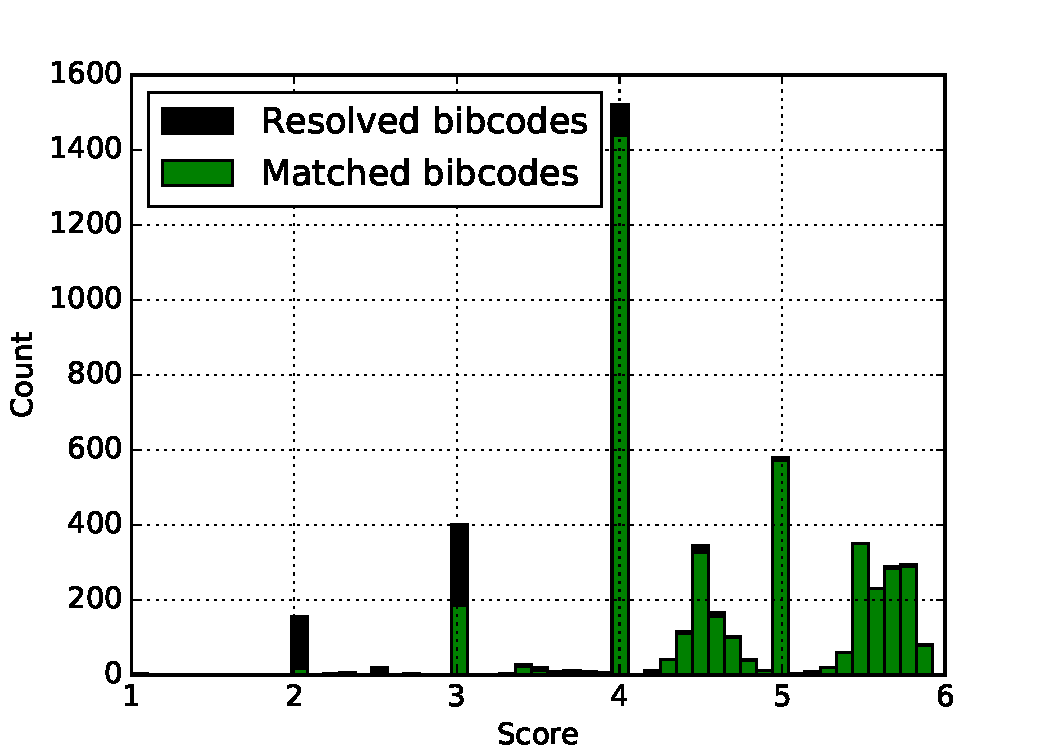
\includegraphics[scale=0.45, trim = 1mm 1mm 1mm 1mm, clip]{Images/refsample_analysed_scores_hist.pdf}
        \par
    \end{centering}
    \caption{Score histogram comparing the total resolved bibcodes (black) with those that match the expected bibcode (green).}
	\label{fig:score_histogram}
\end{figure}




\section{Future improvements}

The tests using around 6\,000 entries demonstrated the good performance of the service with a success ratio greater than 74\%. It also helped to identify a list of improvements that can be performed to increase the number of successfully resolved bibcodes:

\begin{itemize}
	\item Make ADS API Search consider synonyms for author searches or find an alternative solution.
	\item Investigate the entries that lead to a network connection problem since some of them could be linked to the use of string with non conventional characters that are not properly encoded.
	\item Improve authors pattern identification to reduce failed reference string resolutions.
	\item Implement a smarter way of isolating journal name in the reference string.
	\item Consider multiple years if more than one is found.
	\item Accept ADS searches without a year constraint.
\end{itemize}



\bibliographystyle{unsrt}
\bibliography{References}


\end{document}
